\documentclass[a4paper,12pt]{extarticle} \usepackage[utf8]{inputenc}
\usepackage[T1]{fontenc}
\usepackage[margin=2.5cm]{geometry}

% Fonte Caladea se existir, senão lmodern
\IfFileExists{caladea.sty}{
  \usepackage{caladea}
}{
  \usepackage{lmodern} }
\usepackage{ragged2e}
\usepackage{graphicx}
\usepackage{hyperref}
\usepackage{fancyhdr}
\usepackage{xcolor}
\usepackage{rotating}
\usepackage{titlesec}
\usepackage{dirtytalk}
\usepackage[portuguese]{babel}
\usepackage{indentfirst} % Indenta o primeiro parágrafo após seções

% Ajuste do recuo de parágrafo
\setlength{\parindent}{1.5em}

% Centralizar títulos
\titleformat{\section}
  {\normalfont\centering\bfseries\Large}{\thesection}{1em}{}

\titleformat{\subsection}
  {\normalfont\centering\bfseries\large}{\thesubsection}{1em}{}

\titleformat{\subsubsection}
  {\normalfont\centering\bfseries}{\thesubsubsection}{1em}{}

% -------------- Símbolos de Versículo e Resposta --------------
% Definição do símbolo (a “barrinha” inclinada)
\makeatletter
\newcommand{\vers@resp@sym}{%
  \raisebox{0.2ex}{\rotatebox[origin=c]{-20}{$\m@th\rceil$}}%
}
% macro interna que sobrepõe a barrinha e a letra V ou R
\newcommand{\vers@resp}[2]{%
  {\ooalign{%
     \hidewidth\kern#1\vers@resp@sym\hidewidth\cr
     #2\cr
  }}%
}
% comandos públicos \versicle e \response
\DeclareRobustCommand{\versicle}{\vers@resp{-0.1em}{V}}
\DeclareRobustCommand{\response}{\vers@resp{0pt}{R}}
\makeatother
% ^------------- Símbolos de Versículo e Resposta -------------^

% Rodapé com imagem e página
\pagestyle{fancy}
% ---- Cabeçalho ------------
\fancyhf[C]{}
% ----- Rodapé --------------
\fancyfoot[LO,LE]{%
  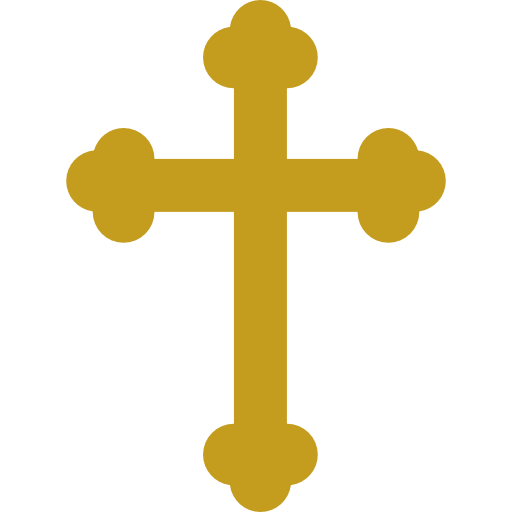
\includegraphics[scale=0.2]{assets/cross.png}\quad
  \textit{Novena a \textbf{Nossa Senhora dos Anjos}}
}
\fancyfoot[RO,RE]{\thepage}

\begin{document}

\begin{center}
  \textbf{\LARGE Novena a Nossa Senhora dos Anjos}\\[0.5em]
  \say{Ó Nossa Senhora dos Anjos, na pequena Igreja da Porciúncula, São Francisco recebeu as vossas bênçãos generosas juntamente com sua Ordem. Ele depositara na vossa presença materna uma grande confiança e devoção, sendo atendido em seus pedidos. Continuai a dispensar os vossos favores sobre nós e sobre nossas necessidades particulares. Nós vos suplicamos, dai-nos a graça da penitência dos pecados, a correção de nossas más inclinações e fortalecimento nos momentos de fraqueza. Quantos recusam a salvação e preferem caminhar nas trevas do erro! Tudo é possível para aquele que crer, para aquele que se arrepender! Vós, ó Mãe, manifestastes a São Francisco o grande desejo de reconciliar os pecadores com Jesus, que se entregou em uma cruz para nos salvar.}\\
\end{center}

\tableofcontents
\thispagestyle{empty}

% --- Vida / Origem da Novena ---
\newpage

\section{Origem da Devoção}

A história da igreja de Nossa Senhora dos Anjos da Porciúncula é um capítulo importante da vida de Giovanni di Pietro di Bernardone, que ficaria mundialmente conhecido como São Francisco de Assis. Este Santo homem, pequeno em estatura, humilde no pensamento e menor por vocação, “escolheu para si e para os seus um pedacinho do mundo, enquanto aqui tinha de viver, pois não poderia servir a Cristo sem ter alguma coisa do mundo. E não foi sem presciência do oráculo divino que o lugar se chamou Porciúncula (pequena porção) desde os tempos antigos, lugar que deveria caber por sorte àqueles que deste mundo não queriam ter quase nada”1.
Conheça a belíssima história de São Francisco com a igreja de Nossa Senhora dos Anjos da Porciúncula.

Nele foi construída uma igreja dedicada a Santíssima Virgem Maria, que por sua humildade singular mereceu ser cabeça de todos os santos logo depois de seu Filho. Em Santa Maria dos Anjos teve início a Ordem dos Frades Menores, aí se levantou a nobre estrutura de inumerável multidão de irmãos, como que sobre um fundamento estável. “O santo teve uma preferência especial por esse lugar, quis que os frades o venerassem de maneira toda particular e quis que fosse conservado como espelho de toda a sua Ordem na humildade e na altíssima pobreza, deixando sua propriedade para outros e reservando para si e para os seus apenas o uso”2.

\subsection{As três igrejas reformadas por São Francisco}

São Francisco recebeu de Cristo a ordem de restaurar a sua Igreja e literalmente restaurou três igrejas. O Pai Seráfico primeiramente restaurou a igreja de São Damião. Como filho autêntico da obediência, pôs-se a trabalhar e a mendigar o material necessário para a reforma. “Por amor de Cristo pobre e crucificado, ele vai pedindo esmola sem qualquer vergonha junto àqueles mesmos que o haviam conhecido como grande senhor”3. Apesar de fraco e extenuado pelos severos jejuns que aplicava a si mesmo, carregava nas costas pesados fardos de pedras. Com a ajuda de Deus e a cooperação do povo, Francisco conseguiu enfim terminar a restauração da igreja de São Damião. Para não ficar de braços cruzados, começou e terminou a reconstrução de outra igreja, dedicada a São Pedro, situada bem distante da cidade de Assis. Mas, o Reconstrutor da Igreja ainda não havia terminado a sua obra-prima.

Depois de reconstruir a igreja de São Pedro, Francisco chegou a um lugar chamado Porciúncula, onde existia uma velha igreja dedicada a Virgem Mãe de Deus, que estava abandonada, sem ninguém que dela cuidasse. “Francisco era grande devoto de Maria Senhora do Mundo, e quando viu a igreja naquele desamparo, começou a morar aí permanentemente a fim de poder restaurá-la”4. O Santo foi agraciado com a visita frequente dos santos anjos, o que aliás não estranhava, uma vez que a igreja se chamava Santa Maria dos Anjos. Ele se fixou neste local por causa de seu respeito pelos anjos e de seu amor a Mãe de Jesus. “Sempre amou esse lugar acima de qualquer outro no mundo, pois foi aí que ele principiou humildemente, progrediu na virtude e atingiu a culminância da felicidade. Foi esse lugar que ele confiou aos Irmãos ao morrer como particularmente caro a Santíssima Virgem”5.

A respeito da pequena igreja de Nossa Senhora dos Anjos, um dos frades menores teve uma visão antes de sua conversão. “Viu ele em volta dessa igreja uma multidão incalculável de pobres cegos, de joelhos, braços erguidos e semblantes voltados para o céu; com gritos e lágrimas, imploravam todos misericórdia e a luz dos olhos. E eis que uma luz brilhante desceu do céu e os envolveu a todos restituindo-lhes a visão e a saúde que almejavam”6. Neste lugar santo, Francisco fundou a Ordem dos Frades Menores, por inspiração de Deus. A divina Providência fez o Pobre de Assis restaurar três igrejas antes de fundar a Ordem e começar a pregar o Evangelho. Francesco progrediu das coisas materiais em direção às realizações mais espirituais, das coisas menores às maiores, na devida ordem. Tudo isso foi sinal profético da obra que Francisco realizaria mais tarde, pela Providência de Deus. Pois, “a Igreja que devia restaurar não era a de pedra, mas a própria Igreja de Cristo, enfraquecida na época pelas divisões, heresias e pelo apego de seus líderes às riquezas e ao poder”7.

\subsection{A predileção por Santa Maria dos Anjos da Porciúncula}

Na Porciúncula, se observava a disciplina mais rígida, tanto no silêncio e no trabalho, quanto em todas as outras práticas regulares dos frades. “Ninguém podia entrar, a não ser frades especialmente designados que, reunidos de todas as partes, o santo queria que fossem verdadeiramente devotados a Deus e perfeitos em tudo. Para todas as pessoas seculares, a entrada estava absolutamente fechada. Não queria que os frades que lá moravam, limitados a um certo número, poluíssem seus ouvidos com relacionamento dos seculares, para não deixarem a meditação das coisas celestes, arrastados para coisas inferiores pelos espalhadores de boatos.

Nesse lugar, ninguém podia dizer coisas ociosas, nem narrar as que tinham sido contadas por outros. Quando isso acontecia, aplicava-se ao culpado, para correção, uma pena salutar. Os que ali moravam ocupavam-se, dia e noite, com os louvores divinos, levando uma vida angelical, cujo perfume admirável se espalhava por toda parte”8. O local era muito apropriado para semelhante vivência de fé e de santidade, pois, conforme diziam os antigos moradores, também se chamava Santa Maria dos Anjos. São Francisco dizia que lhe tinha sido revelado por Deus que Nossa Senhora tinha uma particular predileção por aquele lugar entre todas as outras igrejas construídas no mundo em sua honra. Por isso, o Santo gostava mais dela que de outras igrejas.

O Pobre de Assis, no final de sua vida terrena, dois anos depois de receber os estigmas sagrados, vinte anos após sua conversão, “trabalhado sob os golpes redobrados das angústias e enfermidades, como pedra destinada a entrar na construção da Jerusalém celeste, batido pelo martelo de múltiplas tribulações, devia ser elevado ao cume da perfeição”9. Percebendo que se aproximava o fim de sua vida aqui na Terra, Francisco pediu que o conduzissem a Santa Maria dos Anjos da Porciúncula, a fim de exalar o seu último suspiro, naquele lugar onde anos antes recebera tão abundantemente os dons do Espirito. São Francisco de Assis tinha um amor indizível pela Mãe de Cristo, porque fez nosso Irmão o Senhor da majestade. O Pobre de Assis consagrava a Virgem dos Anjos louvores especiais, orações, afetos, tantos e tais que nenhuma língua humana poderia contar. Para grande alegria dos franciscanos, o Servo dos Leprosos constituiu Nossa Senhora como Advogada da sua Ordem e, à sua proteção e guia, confiou até o fim os filhos que ia deixar à Advogada dos pobres.


\newpage
\section{Orações}

\subsection{Oração Inicial} \label{oracao-inicial}

\textbf{Em nome do Pai, do Filho e do Espírito Santo. Amém.}

Santa Virgem Maria, não há mulher nascida no mundo semelhante a Vós. Filha e serva do altíssimo Rei e Pai celestial. Mãe de nosso santíssimo Senhor Jesus Cristo, esposa do Espírito Santo. Rogai por nós com são Miguel arcanjo e todas as Virtudes do céu e todos os santos junto a vosso santíssimo e dileto filho, nosso Senhor e Mestre. Amém.

% --- Orações Diárias ---

\subsection{Novena em Honra de Nossa Senhora dos Anjos}

\subsubsection{Primeiro Dia}

\noindent

\textbf{Começar com a \nameref{oracao-inicial}.}

Ó Nossa Senhor dos anjos, nós recorremos à vossa materna proteção; Vós que sois a Mãe de Deus e da Mãe da Igreja. Diante de vosso filho Salvador, intercedei por nós, que somos peregrinos neste mundo. Aos pés da Cruz, Vós recebestes a missão de ser Mãe de todo o gênero humano. Ensinai-nos a realizar a vontade do Pai e defendei-nos de todos os males.

\textbf{Finalizar com a \nameref{oracao-final}.}


\subsubsection{Segundo Dia}

\textbf{Começar com a \nameref{oracao-inicial}.}

Ó Virgem Maria, professamos com nossa fé, a vossa Santa e Imaculada Conceição. O Todo-Poderoso vos preservou do pecado, desde a vossa concepção, em função dos méritos de Jesus Cristo. Sabemos que o pecado destrói a comunidade humana e é a causa de todos os males: guerras, divisões e injustiças. Ó Virgem pura, dai-nos a pureza de coração e a retidão em nossas intenções, a fim de que sejamos mais felizes aqui na terra e no céu.

\textbf{Finalizar com a \nameref{oracao-final}.}


\subsubsection{Terceiro Dia}

\textbf{Começar com a \nameref{oracao-inicial}.}

\subsubsection*{Amor a Deus de Nossa Senhora dos Anjos}

Santa Maria, nós confessamos que vós sois a Mãe de Deus, a Mãe de Jesus, a Esposa do Espírito Santo. Cremos na Vossa Maternidade Divina. Com toda a generosidade, vós nos oferecestes o Salvador do mundo. Nos vossos braços, Jesus é oferenda pura. Fazei, ó Virgem Mãe, que jamais nos afastemos de vosso amado filho, por mais difícil que seja a caminhada, mas estejamos prontos a levar a chama viva da fé e da felicidade em direção à pátria definitiva, o céu.

\textbf{Finalizar com a \nameref{oracao-final}.}


\subsubsection{Quarto Dia}

\textbf{Começar com a \nameref{oracao-inicial}.}

“Eis aqui a serva do Senhor, faça-se em mim segundo a Vossa Palavra”. Toda a vossa vida, Maria foi construída em realizar a vontade de Deus, a responder a um chamado tão sublime, não somente com palavra, pois a vossa vida inteira tornou-se uma só resposta de obediência.

A Palavra de Deus, contida na Bíblia, é luz, é vida, é salvação. Hoje, ó Virgem Rainha dos anjos, ensinai-nos a acolher, com generosidade a palavra do vosso Filho em nossos corações como Vós acolhestes no dia da Anunciação. Queremos também ser fieis discípulos de Jesus Cristo

\textbf{Finalizar com a \nameref{oracao-final}.}


\subsubsection{Quinto Dia}

\textbf{Começar com a \nameref{oracao-inicial}.}


Com toda a confiança. Nós Vos suplicamos, ó virgem Mãe, amparai de uma maneira especial, as nossas famílias; fazei que elas tenham como modelo de vida a Família de Nazaré, que apesar de conhecer as dificuldades, o trabalho de cada dia, a pobreza, permanecia unida no amor, na compreensão e na fé. Não deixeis a divisão abalar os alicerces de nossos lares. Que em nossas mesas jamais falte o pão necessário, fruto do trabalho e dom da Providência. Conduzi os esposos na unidade, as crianças e os jovens através de uma educação sólida e cristã. Sede a Rainha de todas as famílias e da nossa cidade. Confiamos na vossa proteção, hoje e sempre.

\textbf{Finalizar com a \nameref{oracao-final}.}


\subsubsection{Sexto Dia}

\textbf{Começar com a \nameref{oracao-inicial}.}


Salve, ó Rainha dos Anjos! Salve, ó rainha nossa!  Somos felizes por termos recebido do Pai uma Mãe cheia de graça, cheia de amor e disponibilidade para nos dirigir e nos orientar. Toda a vossa vida se resumiu em servir, em acolher, em confortar aqueles eu sofrem, enfim, em amar a Deus sobre todas as coisas e ao próximo. Dai-nos a perseverança no caminho do bem e ensinai-nos a sermos verdadeiros seguidores de Jesus Cristo, agora e na hora de nossa morte.


\textbf{Finalizar com a \nameref{oracao-final}.}


\subsubsection{Sétimo Dia}

\textbf{Começar com a \nameref{oracao-inicial}.}

Intercedei por nós, Santíssima Virgem.  A Igreja inteira se prostra após vossos pés, esperando o vosso auxílio. Defendei-a de todos os perigos e das forças malignas. Fortalecei o nosso Papa, o Vigário de Cristo, para conduzir na unidade o seu rebanho. Sede nossa Rainha, o “auxílio dos cristãos”, a “consoladora dos aflitos”. Vós sois a nossa segurança, o nosso estímulo e o nosso exemplo. Fazei que o Evangelho seja anunciado até os confins da terra e todos se disponham a aceitar a salvação trazida por vosso filho.

\textbf{Finalizar com a \nameref{oracao-final}.}


\subsubsection{Oitavo Dia}

\textbf{Começar com a \nameref{oracao-inicial}.}


Glória ao Pai, a Jesus Cristo e ao Espírito Santificador, que realizaram grandes maravilhas em Maria. Não houve nem haverá criatura tão santa, tão sublime e tão radiante como ela. Os anjos e os santos vos louvam, ó Mãe amável. E nós também elevamos os nossos olhos para vós com profunda confiança filial. Sede para vossos filhos um refúgio e amparo, a fim de que cumpramos a nossa missão, e um dia possamos chegar ao céu.


\textbf{Finalizar com a \nameref{oracao-final}.}


\subsubsection{Nono Dia}

\textbf{Começar com a \nameref{oracao-inicial}.}

Ó Nossa senhora dos anjos, na pequena Igreja da Porciúncula, São Francisco recebeu as vossas bênçãos generosas juntamente com sua Ordem. Ele depositara na vossa presença materna uma grande confiança e devoção, sendo atendido em seus pedidos. Continuai a dispensar os vossos favores sobre nós e sobre nossas necessidades particulares. Nós vos suplicamos, dai-nos a graça da penitência dos pecados, a correção de nossas más inclinações e fortalecimento nos momentos de fraqueza. Quantos recusam a salvação e preferem caminhar nas trevas do erro! Tudo é possível para aquele eu crer, para aquele que se arrepender. Vós, ó Mãe, manifestastes a São Francisco o grande desejo de reconciliar os pecados com Jesus, que se entregou em uma cruz, para nos salvar. Rogai por nós. Agora e na hora de nossa morte.

\textbf{Finalizar com a \nameref{oracao-final}.}

% --- Oração Final ---
\newpage
\subsection{Oração Final} \label{oracao-final}

Lembrai-vos, ó piedosíssima Virgem Maria, que nunca se ouviu dizer, que algum daqueles que recorreram à vossa proteção, imploraram a vossa assistência e reclamaram o vosso socorro, fosse por vós desamparado. Animado eu, pois, com igual confiança, a Vós, ó Virgem entre todas singular, como à minha mãe recorro; de vós me valho e gemendo sob o peso de meus pecados, me prostro aos vossos pés. Não rejeiteis as minhas súplicas, ó Mãe do filho de Deus humanado, mas dignai-vos de ouvi-las propícia e de me alcançar o que vos rogo. Amém.

\begin{center}
  \large
  \textbf{Pai-Nosso, Ave-Maria e Glória.}
\end{center}




\vfill

\begin{center}
\subsection*{Fontes:}
\href{https://blog.cancaonova.com/tododemaria/a-historia-de-nossa-senhora-dos-anjos/}{Blog Canção Nova}\\ 
\href{https://ofs-sp.org.br/nossas-fraternidades/}{OFS}
\end{center}


\end{document}
